\documentclass[9pt,serif,mathserif]{beamer}

\usepackage[utf8]{inputenc}

\def\today{\ifcase\month\or
January\or February\or March\or April\or May\or June\or
July\or August\or September\or October\or November\or December\fi
\space \number\year
} % \today of the form "Month Year"

\usetheme[progressbar=frametitle]{metropolis}
\usepackage{appendixnumberbeamer}

\usepackage[square, numbers, comma, sort&compress]{natbib} % Use the natbib reference package - read up on this to edit the reference style; if you want text (e.g. Smith et al., 2012) for the in-text references (instead of numbers), remove 'numbers' 
\bibliographystyle{apsrev4-1-etal} % Use the utphys, apsrev4-1, kp and more BibTeX style for formatting the Bibliography
\usepackage{notoccite}

\usepackage{amsmath,amsfonts,amssymb,amscd,amsthm,xspace,mathtools}
\usepackage[centerlast,small,sc]{caption}
\graphicspath{{Figures/},{../Thesis/Figures/}} % Specifies the directory where pictures are stored

%%% FONTS
\newcommand\hmmax{0}
\newcommand\bmmax{0}
\usepackage{mathpazo}
\usepackage{bm}
\usepackage{tabu}

\DeclareMathAlphabet{\mathpzc}{OT1}{pzc}{m}{it}
\DeclareSymbolFont{cmletters}{OT1}{cmr}{m}{n}
\DeclareMathSymbol{\Upsilon}{\mathalpha}{cmletters}{"7}

\usepackage[bbgreekl]{mathbbol}
\DeclareSymbolFontAlphabet{\mathbb}{AMSb}
\DeclareSymbolFontAlphabet{\mathbbl}{bbold}

\usepackage[mathscr]{euscript}

\newcommand{\lambdabar}{{\mkern 0.0mu\lambda\mkern -8.2mu\mathchar '26\mkern 2mu}}

\newcommand{\dd}{\mathrm{d}}
\newcommand{\uu}[3][]{ {}_{#1} #2_{#3} }
\renewcommand{\Re}{\mathrm{Re}}
\renewcommand{\Im}{\mathrm{Im}}

\setbeamerfont{frametitle}{size=\Large,shape=\scshape}
\setbeamerfont{title page}{size=\Large,shape=\scshape}

%-------------------------------------------------------------------------------------



\title{\scshape\LARGE Aspects of superradiant scattering \\ off Kerr black holes}
%\subtitle{A modern beamer theme}
\date{November 2017}
\author{\textbf{José \textsc{Sá}} \hfill \textit{Supervisor:} João G. \textsc{Rosa} \\[0.15cm] \phantom{arg} \hfill \textit{Co-supervisor:} Orfeu \textsc{Bertolami} \\[0.4cm]}
\institute{Faculdade de Ciências da Universidade do Porto}
% \titlegraphic{\hfill\includegraphics[height=1.5cm]{logo.pdf}}



\begin{document}

\maketitle

% \begin{frame}{Table of contents}
%     \setbeamertemplate{section in toc}[sections numbered]
%     \tableofcontents[hideallsubsections]
% \end{frame}

\begin{frame}[fragile]{Outline}
    \begin{itemize}
        \large
        \setlength\itemsep{1.2em}
        \item What is superradiance ?
        \item Kerr black hole and the Penrose process
        \item Newman-Penrose formalism and the Teukolsky equation
        \item Analytical approximated solutions
        \item Numerical methods
        \item Scattering of planes waves 
        \item Conclusions and future work
    \end{itemize}
\end{frame}

{
    \usebackgroundtemplate{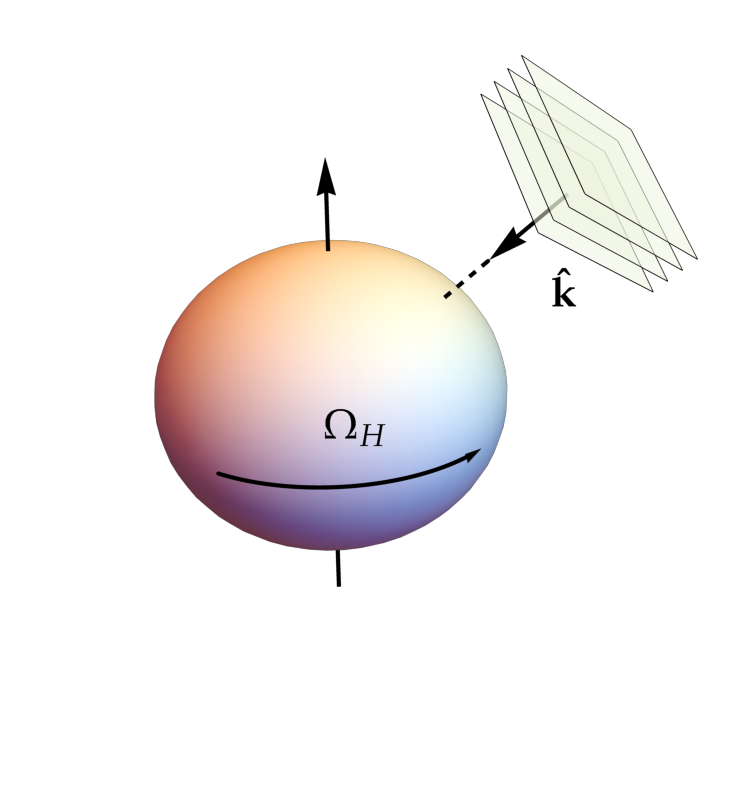
\includegraphics[scale=0.55,trim=-11cm 0 0 -3cm]{test.pdf}}
    \begin{frame}[fragile]{Introduction}

        \begin{columns}[T,onlytextwidth]        
            \column{0.5\textwidth}
        
                \metroset{block=fill}
        
                \begin{block}{Default}
                Block content.
                \end{block}
        
                \begin{alertblock}{Alert}
                Block content.
                \end{alertblock}
        
                \begin{exampleblock}{Example}
                Block content.
                \end{exampleblock}
        
        \end{columns}

    \end{frame}
}

\begin{frame}[fragile]{Kerr black hole}

    \vspace{0.15cm}

    \metroset{block=fill}
    \begin{block}{Boyer-Lindquist coordinates}
        \begin{align*}
            \begin{split}
                \bm{g} = & \left(1 - \frac{2 M r}{\rho^2} \right) \dd t^2 + 2 a \sin^2\theta \frac{(r^2+a^2-\Delta)}{\rho^2} \dd t \dd \varphi \\
                &- \frac{(r^2+a^2)^2- \Delta a^2 \sin^2\theta}{\rho^2} \sin^2\theta \dd\varphi^2 - \frac{\rho^2}{\Delta} \dd r^2 - \rho^2 \dd \theta^2
            \end{split}
        \end{align*}
        \centering
        $[\,\Delta=r^2 - 2 M r + a^2 ~,~~ \rho^2 = r^2 + a^2 \cos^2\theta\,]$
    \end{block}

    \begin{itemize}
        \setlength\itemsep{0.8em}
        \item BH angular momentum $J = a M \quad\left[ a=0 ~\Rightarrow \text{Schwarzschild} \right]$ 
        \item Killing vectors $\bm{k}=\partial_t$ (stationary) and $\bm{m}=\partial_\varphi$ (axisymmetric)
        \item Horizons at $g^{rr}=0 ~\Rightarrow~ \Delta=0 ~\Rightarrow~ r = r_{\pm} \equiv M \pm \sqrt{M^2-a^2}$ \\
        \emph{Cosmic censorship} conjecture $~\Rightarrow~$ $|a| \le M$
        
        \item Infinite redshift boundary $g_{tt}=0 ~\Rightarrow$ \alert{Ergoregion} $(g_{tt}<0)$
        $$r_+<r<r_\mathrm{ergo}(\theta) \equiv M + \sqrt{M^2 - a^2 \cos^2\theta}$$
    \end{itemize}
\end{frame}

\begin{frame}[fragile]{Penrose process}
    \begin{itemize}
        \setlength\itemsep{0.8em}
        \item Particle decays into two inside the ergoregion: $\bm{p} = \bm{p_1} + \bm{p_2}$
        %\vspace{0.2cm}
        \begin{columns}[onlytextwidth]        
            \begin{column}{0.7\textwidth}
                \centering
                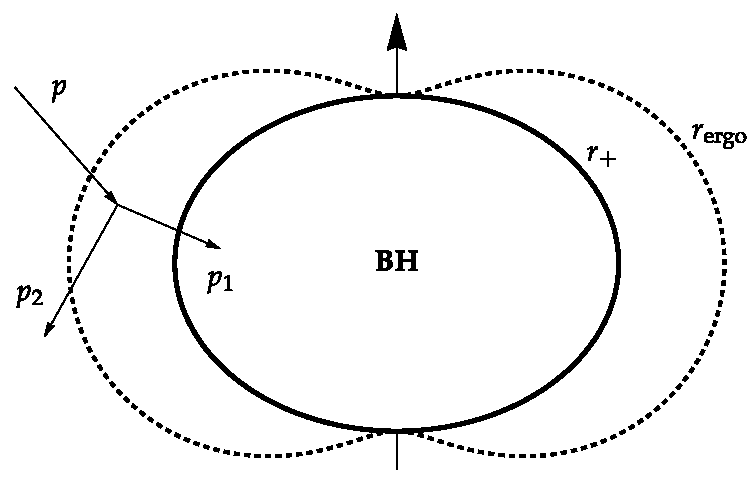
\includegraphics[scale=0.55,trim=0.3cm 0.3cm 0 0.3cm]{ergoPenrose.pdf}
            \end{column}
            \hfill
            \begin{column}{0.26\textwidth}
                \vspace*{0.5cm}
                \metroset{block=fill}
                \begin{block}{\small Killing horizon}
                    \footnotesize Hypersurface $r=r_{+}$ with normal null vector $$\bm{\xi} = \bm{k} + \Omega_H \bm{m} \qquad$$ 
                    
                    Event horizon angular momentum:
                    $$\Omega_H = \frac{a}{2 M r_+} \qquad$$
                \end{block}
            \end{column}
        \end{columns}
        \vspace{0.3cm}
        \item We may have $E_1 = \bm{k} \cdot \bm{p_1} < 0 ~\Rightarrow E_2 = E + |E_1| > E $
        \item Local energy condition $\bm{\xi}\cdot\bm{p_1}>0$ at $r=r_{+} ~\Rightarrow E_1 - \Omega_H \, L_1 > 0$
        $$ \psi \sim e^{-i \omega t + i m \varphi} ~\Rightarrow~ \frac{\delta J}{\delta M} = \frac{\hbar m}{\hbar \omega} ~\Rightarrow~ \delta M < 0 ~\land~ \fbox{ \omega( \omega - \Omega_H \,m) < 0~} $$\\
        \hspace*{5.5cm}\alert{Energy extraction !}
    \end{itemize}
\end{frame}

\begin{frame}{Newman-Penrose formalism}    
    \begin{itemize}
        \setlength\itemsep{1.5em}
        \item Electromagnectic perturbations ($A^\mu \ll 1$)
        \begin{align*}
            R_{\mu\nu} - \frac{R}{2} g_{\mu\nu} &= 8 \pi T_{\mu\nu} = 0 + \mathcal{O}(A^2) ~\Rightarrow\text{fixed background (Kerr)}
        \end{align*}

        \item Tetrad frame of complex null vectors $(\bm{e}_1,\bm{e}_2,\bm{e}_3,\bm{e}_4)
        = (\bm{\mathfrak{l}},\bm{\mathfrak{n}},\bm{\mathfrak{m}},\bar{\bm{\mathfrak{m}}}\equiv \bm{\mathfrak{m}}^*)$
        with $\bm{\mathfrak{l}}\cdot\bm{\mathfrak{m}} = \bm{\mathfrak{n}}\cdot\bm{\mathfrak{m}} = 0 ~,~~ \bm{\mathfrak{l}}\cdot\bm{\mathfrak{n}} = 1 ~,~~ \bm{\mathfrak{m}}\cdot\bar{\bm{\mathfrak{m}}} = -1$
        \begin{equation*}
            \underbrace{\mathbf{E} ~,~ \mathbf{B}}_\text{6 real components}
            \quad\longrightarrow\quad
            \boxed{
            \begin{aligned}
                \phi_0 &= F_{\mu\nu} \mathfrak{l}^\mu \mathfrak{m}^\nu \\
                \phi_1 &= \tfrac{1}{2} F_{\mu\nu} ( \mathfrak{l}^\mu \mathfrak{n}^\nu - \mathfrak{m}^\mu \bar{\mathfrak{m}}^\nu ) \\
                \phi_2 &= F_{\mu\nu} \bar{\mathfrak{m}}^\mu \mathfrak{n}^\nu 
            \end{aligned}
            }
            %\quad\text{and}\quad\text{c.c.} \Leftrightarrow (\bm{\mathfrak{m}}%\rightleftarrows \bar{\bm{\mathfrak{m}}})
        \end{equation*}

        \item Equations written using tetrad derivatives $(\mathbbl{D}, \mathbbl{\Delta}, \bbdelta, \bar{\bbdelta})$ and spin connection $\gamma_{cab} = (e_c)^\mu (e_b){}^\nu \nabla_\nu (e_a)_{\mu} ~\Rightarrow~ \lambda, \pi, \tau, \varrho, \varepsilon, \sigma,\kappa, \gamma ,\mu, \nu, \alpha,\beta$
        \begin{equation*}
            \begin{aligned}[c]
                \nabla_\mu F^{\mu\nu} &= 0 \\
                \nabla_{[\mu} F_{\nu\rho]} &= 0
            \end{aligned}
            \quad\longrightarrow~\left\{~~
            \begin{aligned}[c]
                \mathbbl{D} \phi_2 - \bar{\bbdelta} \phi_1 &= -\lambda \phi_0 + 2 \pi \phi_1 + (\varrho - 2 \varepsilon) \phi_2 \\
                \mathbbl{\Delta} \phi_1 - \bbdelta \phi_2 &= \nu \phi_0 - 2 \mu \phi_1 + (2\beta-\tau) \phi_2 \\
                \mathbbl{D} \phi_1 - \bar{\bbdelta} \phi_0 &= (\pi - 2 \alpha) \phi_0 + 2 \varrho \phi_1 - \kappa \phi_2 \\
                \mathbbl{\Delta} \phi_0 - \bbdelta \phi_1 &= (2 \gamma - \mu) \phi_0 - 2 \tau \phi_1 + \sigma \phi_2
            \end{aligned}
            \right.
        \end{equation*}
    \end{itemize}
\end{frame}

\begin{frame}[fragile]{Newman-Penrose formalism}
    \metroset{block=fill}
    \begin{block}{Kinnersley tetrad}
        \begin{columns}[onlytextwidth]   
            \begin{column}{0.5\textwidth}
                \begin{align*}
                    \bm{\mathfrak{l}} &= \frac{1}{\Delta} \Big( r^2+a^2, \,\Delta, \,0, \,a \Big) \\
                    \bm{\mathfrak{n}} &= \frac{1}{2 \rho^2} \Big( r^2+a^2, -\Delta, \,0, \,a \Big) \\
                    \bm{\mathfrak{m}} &= \frac{1}{\sqrt{2} \bar{\rho}} \Big( i \,a \sin\theta, \,0, \,1, \,i \csc\theta \Big) \\[0.3cm]
                    & ~~ [\,\bar{\rho} = r + i \,a \cos\theta \,]
                \end{align*}
            \end{column}
            \begin{column}{0.5\textwidth}
                \begin{itemize}
                    \item $\bm{\mathfrak{l}}$, $\bm{\mathfrak{n}}$ are the doubly degenerate principal null of directions of the Weyl tensor
                    \begin{align*}
                        \bm{\mathfrak{l}} &\sim (\bm{e}_t + \bm{e}_r)
                        \qquad\text{(ingoing)} \\
                        \bm{\mathfrak{n}} &\sim \tfrac{1}{2}(\bm{e}_t - \bm{e}_r) 
                        \quad\text{(outgoing)}
                    \end{align*}
                    \item $\bm{\mathfrak{l}}$, $\bm{\mathfrak{n}}$ are geodesic ($\kappa = \lambda=0$) \\ and shear-free ($\nu=\sigma=0$) \\ 
                    $~~\Rightarrow$ \alert{equations decouple}
                \end{itemize}
            \end{column}
        \end{columns}
    \end{block}
    \begin{itemize}
        \item Reformulation of the fields: $\quad\Phi_n = (\sqrt{2} \bar{\rho})^n \,\phi_n \quad (n=0,1,2)$
        \item Spacetime symmetry $~\Rightarrow~ \Phi_n \sim e^{-i\omega t + i m \phi}  ~\Rightarrow~ \partial_t \rightarrow -i\omega ~,~ \partial_\varphi \rightarrow i m$ 
        \item Rewrite operators: $\mathbbl{D} = \mathscr{D}_0 ~,~ \mathbbl{\Delta} = - \frac{\Delta}{2 \rho^2 }\mathscr{D}^\dagger_0$   
    \end{itemize}
\end{frame}

\begin{frame}[fragile]{Newman-Penrose formalism}
    \begin{verbatim}The theme provides sensible defaults to
\emph{emphasize} text, \alert{accent} parts
or show \textbf{bold} results.\end{verbatim}

\begin{center}becomes\end{center}

The theme provides sensible defaults to \emph{emphasize} text,
\alert{accent} parts or show \textbf{bold} results.
\end{frame}

\begin{frame}{Newman-Penrose formalism}
    %\metroset{block=fill}
    \begin{block}{\hspace{1.0cm}\alert{Coordinate frame}\hspace{3.5cm}\alert{Tetrad frame}}
        \vspace{0.45cm}
        \begin{columns}[T,onlytextwidth]        
            \begin{column}{0.5\textwidth}
                \begin{itemize}
                    \item Vector (coordinate) basis
                    $$\bm{e}_\mu \equiv \frac{\partial}{\partial x^\mu} \quad (\mu = t,r,\theta,\varphi)$$
                    \item Spacetime metric
                    $$g_{\mu\nu}$$
                    \item Tensorial components
                    $$ A_\mu ~,~ F_{\alpha\beta} $$
                    \item Covariant derivative
                    $$ A_{\mu;\nu} = A_{\mu,\nu} - \Gamma_{\mu\nu}^\rho \,A_\rho $$
                    \item Levi-Civita connection
                    $$\Gamma^\rho_{\mu\nu} = \tfrac{1}{2} g^{\rho\sigma} (g_{\sigma\mu,\nu}+g_{\sigma\mu,\nu}-g_{\mu\nu,\sigma})$$
                \end{itemize}
            \end{column}
            \vrule{}
            \begin{column}{0.5\textwidth}
                \begin{itemize}
                    \item Tetrad (non-coordinate) basis
                    $$ \bm{e}_a \equiv (e_a)^\mu \frac{\partial}{\partial x^\mu} \quad (a = 1,2,3,4)$$
                    \item Raising/lowering tetrad indices
                    $$\eta_{ab} = \bm{e}_a \cdot \bm{e}_b = (e_a)^\mu (e_b)^\nu g_{\mu\nu} $$
                    \item Tetrad (NP) scalars
                    $$ A_a = (e_a)^\mu \,A_\mu ~,~ F_{ab} = (e_a)^\alpha (e_b)^\beta F_{\alpha\beta} $$
                    \item Intrinsic derivative
                    $$ A_{a|b} \equiv (e_a)^\mu (e_b)^\nu A_{\mu;\nu} = A_{a,b} - \gamma_{cab} \,A^c $$
                    \item Spin connection
                    $$\gamma_{cab} = (e_c)^\mu (e_a)_{\mu;\nu} A_{\mu;\nu} = (e_b){}^\nu$$
                \end{itemize}
            \end{column}
        \end{columns}
        \vspace{0.15cm}
    \end{block}
\end{frame}

\begin{frame}{Newman-Penrose formalism}
    \begin{block}{Kinnersley tetrad}
        \begin{align*}
            \bm{\mathfrak{l}} &= \frac{1}{\Delta} \Big( r^2+a^2, \,\Delta, \,0, \,a \Big) \\
            \bm{\mathfrak{n}} &= \frac{1}{2 \rho^2} \Big( r^2+a^2, -\Delta, \,0, \,a \Big)\\
            \bm{\mathfrak{m}} &= \frac{1}{\sqrt{2} \bar{\rho}} \Big( i a \sin\theta, \,0, \,1, \,i \csc\theta \Big)
        \end{align*}
    \end{block}
    \begin{align*}
        \uu[\pm1]{Z}{\ell m} &\simeq  - 4 \bar{\omega} (\bar{\omega} - m \bar{\Omega}_H) \,(2-\tau)(2\bar{\omega} \tau)^{2\ell} \\
        & \qquad\qquad \times \left[\frac{(\ell-1)! (\ell+1)!}{(2\ell)! (2\ell+1)!}\right]^2 \prod_{n=1}^{\ell}\left(n^2 + \frac{4 \varpi^2}{\tau^2} \right)
    \end{align*}
\end{frame}

\begin{frame}[fragile]{Typography}
        \begin{verbatim}The theme provides sensible defaults to
\emph{emphasize} text, \alert{accent} parts
or show \textbf{bold} results.\end{verbatim}

    \begin{center}becomes\end{center}

    The theme provides sensible defaults to \emph{emphasize} text,
    \alert{accent} parts or show \textbf{bold} results.
\end{frame}

\begin{frame}{Font feature test}
    \begin{itemize}
    \item Regular
    \item \textit{Italic}
    \item \textsc{SmallCaps}
    \item \textbf{Bold}
    \item \textbf{\textit{Bold Italic}}
    \item \textbf{\textsc{Bold SmallCaps}}
    \item \texttt{Monospace}
    \item \texttt{\textit{Monospace Italic}}
    \item \texttt{\textbf{Monospace Bold}}
    \item \texttt{\textbf{\textit{Monospace Bold Italic}}}
    \end{itemize}
\end{frame}

\begin{frame}{Lists}
    \begin{columns}[T,onlytextwidth]
    \column{0.33\textwidth}
        Items
        \begin{itemize}
        \item Milk \item Eggs \item Potatos
        \end{itemize}

    \column{0.33\textwidth}
        Enumerations
        \begin{enumerate}
        \item First, \item Second and \item Last.
        \end{enumerate}

    \column{0.33\textwidth}
        Descriptions
        \begin{description}
        \item[PowerPoint] Meeh. \item[Beamer] Yeeeha.
        \end{description}
    \end{columns}
\end{frame}

\begin{frame}{Animation}
    \begin{itemize}[<+- | alert@+>]
    \item \alert<4>{This is\only<4>{ really} important}
    \item Now this
    \item And now this
    \end{itemize}
\end{frame}


\begin{frame}{Blocks}
    Three different block environments are pre-defined and may be styled with an
    optional background color.

    \begin{columns}[T,onlytextwidth]
    \column{0.5\textwidth}
        \begin{block}{Default}
        Block content.
        \end{block}

        \begin{alertblock}{Alert}
        Block content.
        \end{alertblock}

        \begin{exampleblock}{Example}
        Block content.
        \end{exampleblock}

    \column{0.5\textwidth}

        \metroset{block=fill}

        \begin{block}{Default}
        Block content.
        \end{block}

        \begin{alertblock}{Alert}
        Block content.
        \end{alertblock}

        \begin{exampleblock}{Example}
        Block content.
        \end{exampleblock}

    \end{columns}
\end{frame}

\begin{frame}{Math}
    \begin{equation*}
    e = \lim_{n\to \infty} \left(1 + \frac{1}{n}\right)^n
    \end{equation*}
\end{frame}

\begin{frame}{Quotes}
    \begin{quote}
    Veni, Vidi, Vici
    \end{quote}
\end{frame}

{%
\setbeamertemplate{frame footer}{My custom footer}
\begin{frame}[fragile]{Frame footer}
    Metropolis defines a custom beamer template to add a text to the footer. It can be set via
    \begin{verbatim}\setbeamertemplate{frame footer}{My custom footer}\end{verbatim}
\end{frame}
}

\section{Conclusion}

\begin{frame}{Summary}

    Get the source of this theme and the demo presentation from

    \begin{center}\url{github.com/matze/mtheme}\end{center}

    The theme \emph{itself} is licensed under a
    \href{http://creativecommons.org/licenses/by-sa/4.0/}{Creative Commons
    Attribution-ShareAlike 4.0 International License}.

    \begin{center}\ccbysa\end{center}

\end{frame}

{
    \setbeamercolor{palette primary}{fg=black, bg=yellow}
    \begin{frame}[standout]
        Questions?
    \end{frame}\begin{frame}{Line plots}
        
        \end{frame}
        \begin{frame}{Bar charts}
        
        \end{frame}
}

\appendix

\begin{frame}[fragile]{Backup slides}
    Sometimes, it is useful to add slides at the end of your presentation to
    refer to during audience questions.

    The best way to do this is to include the \verb|appendixnumberbeamer|
    package in your preamble and call \verb|\appendix| before your backup slides.

    Metropolis will automatically turn off slide numbering and progress bars for
    slides in the appendix \cite{Rosa2017}.
\end{frame}

\begin{frame}[allowframebreaks]{References}

    \bibliography{../Bibliography}

\end{frame}

\end{document}